\section{Proposed Solution}
\begin{frame}{Proposed Solution}
    \begin{center}
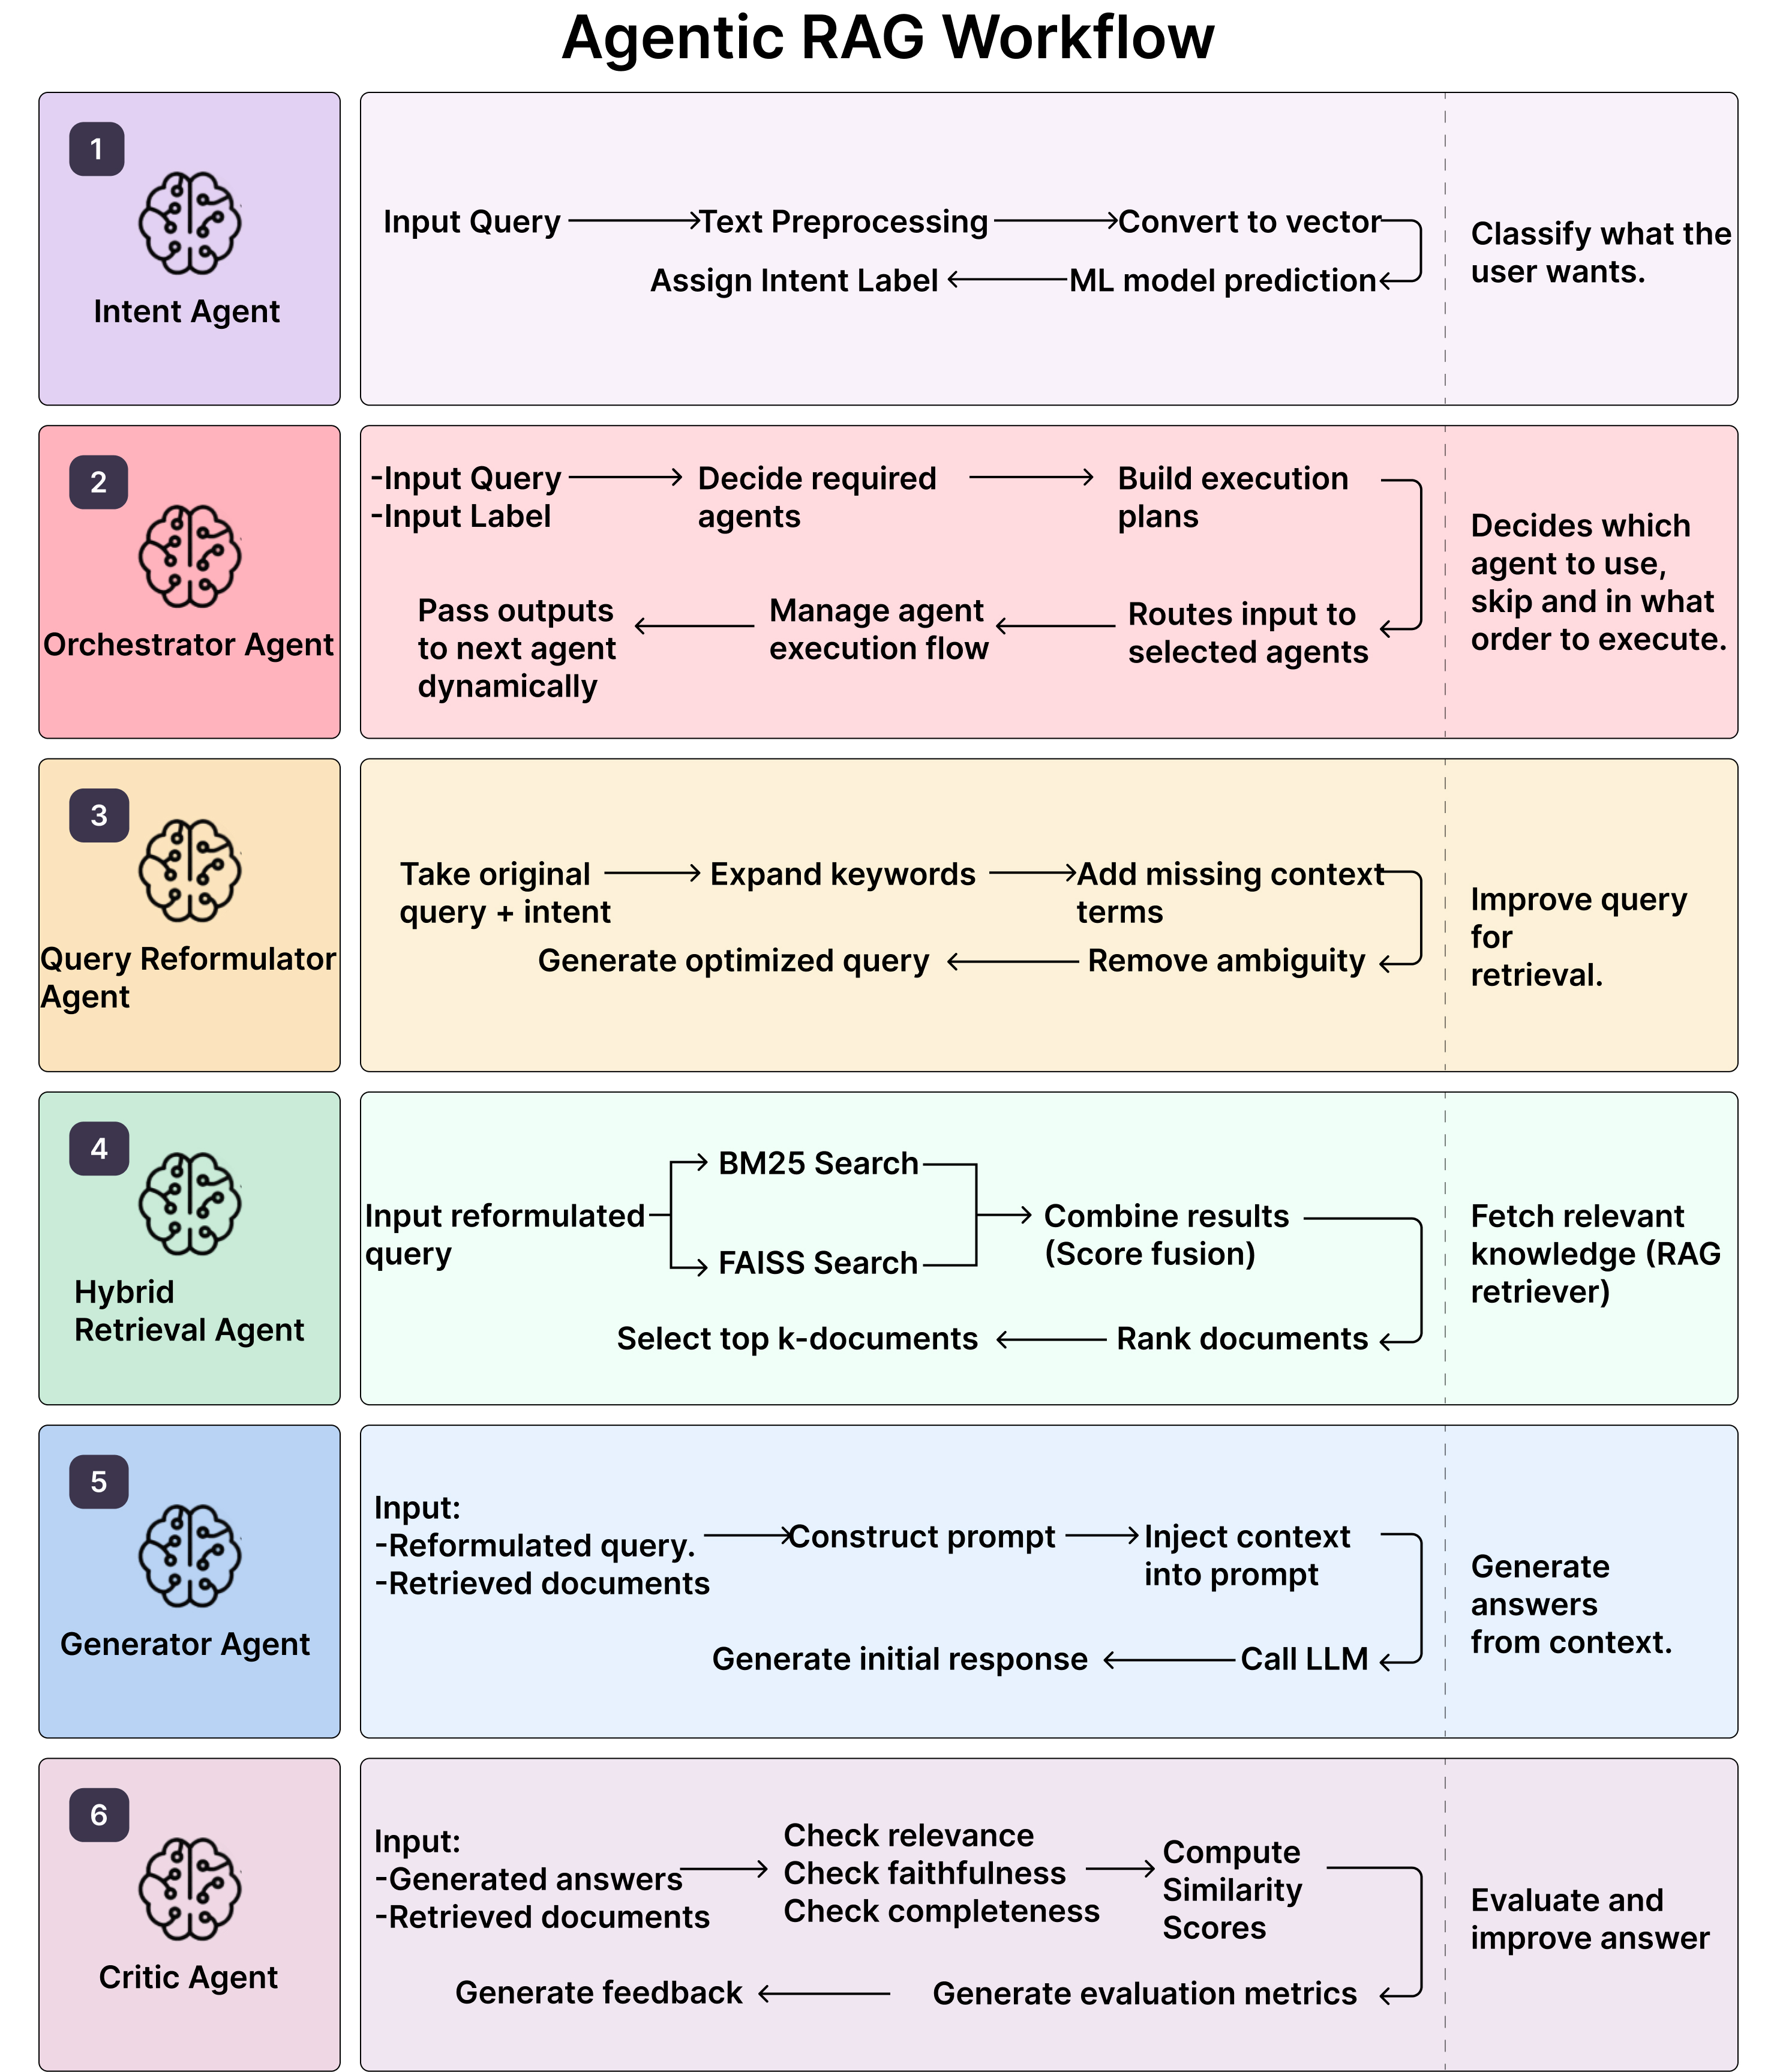
\includegraphics[width=1.5\textwidth,height=.85\textheight,keepaspectratio]{slides/Agentic RAG Workflowjpg.jpg}
\end{center}
\end{frame}

\begin{frame}{Proposed Solution...}
    To address the limitations of existing RAG systems - fragmented pipelines, retrieval instability, weak evaluation, and poor generalisability - we propose an Agentic RAG framework with \textbf{RRF}-based Hybrid Retrieval. Rather than a single-pass pipeline, the system uses a set of specialised agents that collaborate, verify, and self-correct at each stage.
\vspace{0.8em}
    \begin{itemize}
        \item \textbf{Intent Agent - understanding what the user actually wants}
        Instead of treating the raw query as-is, the Intent Agent first preprocesses the text, converts it to a vector, and classifies the user's intent - for example, whether the query is informational, technical, or navigational. This directly addresses the limitation of data and query quality dependency, ensuring the system understands the goal before searching.

    \end{itemize}
\end{frame}

\begin{frame}{Proposed Solution...}
    \begin{itemize}
        \item \textbf{Orchestrator Agent - deciding who does what and in what order}

        This is the brain of the pipeline. The Orchestrator receives both the raw query and the intent label, then dynamically decides which agents to activate, in what sequence, and whether any can be skipped. It builds an execution plan, routes inputs to the appropriate agents, manages the flow between them, and passes outputs forward. No existing literature implements this kind of dynamic coordination - systems in prior work follow fixed, linear pipelines with no ability to adapt the execution path based on query type or context.

        
         \item \textbf{Query Reformulation Agent - improving the query before retrieval}
         
            Using the detected intent, this agent expands keywords, adds missing context, and rewrites the query into a cleaner, more precise form. This tackles the methodological gap in existing systems where queries are fed directly into search without any preprocessing, often producing noisy or irrelevant results.

        

    \end{itemize}
\end{frame}

\begin{frame}{Proposed Solution...}
    \begin{itemize}
        \item \textbf{Hybrid Retrieval Agent with RRF}
        
        The reformulated query is run through two parallel search methods - BM25 [10] (keyword/lexical search) and FAISS (semantic/vector search). Their results are then merged using \textbf{RRF}, which re-ranks documents by combining scores from both methods without needing to normalise them. This produces a more stable, accurate, and comprehensive ranked list - directly solving the retrieval instability and the cost-quality tradeoff that plague existing architectures.
    
         \item \textbf{Generator Agent - synthesising the answer from retrieved context}
         
            The top-ranked documents are passed to the Generator Agent, which injects them as context into an \textbf{LLM} prompt and produces an initial response. The agent is explicitly instructed to cite sources and avoid hallucination - grounding the answer entirely in the retrieved documents rather than the model's internal (and potentially outdated) knowledge.


    \end{itemize}
\end{frame}

\begin{frame}{Proposed Solution...}
    \begin{itemize}
        \item \textbf{Critic Agent with real evaluation metrics - verifying quality before returning}
        
        Unlike existing systems that produce an answer and stop, our Critic Agent evaluates the generated answer across three dimensions - Faithfulness, Relevance, and Completeness - using both \textbf{LLM}-based scoring and token-level F1. If the answer fails, the agent feeds back the reason and triggers a new retrieval-generation cycle. This closes the evaluation gap that existing literature ignores and ensures end-to-end quality rather than isolated module performance.
    \end{itemize}
\end{frame}